
\paragraph{\acs{meteor}}
% Its values range from 0 to 1 \citep{kurt_pehlivanoglu_comparative_2024}.
\ac{meteor} was proposed to address the limitations of \ac{bleu}. 
Unlike \ac{bleu}, \ac{meteor} explicitly incorporates recall. 
Although \ac{meteor} also captures semantic aspects through stemming and synonym matching modules, we consider  primarily a syntactic metric~\citep{kurt_pehlivanoglu_comparative_2024}. 

The order of \ac{meteor}'s modules reflects their priority in the alignment process. 
If the first module is exact matching, all possible mappings of candidate word unigrams to exact matches in the reference text are considered. 
Although valid alignments may restrict each unigram to a single mapping, multiple mappings are allowed in this initial stage. 
In the second stage, the best subset of unigram mappings is selected according to cardinality and minimal crossing.
Crossings are intersection of matchings and illustrated in \Cref{fig:meteor_crossings}.

\begin{figure}[h]
    \centering
    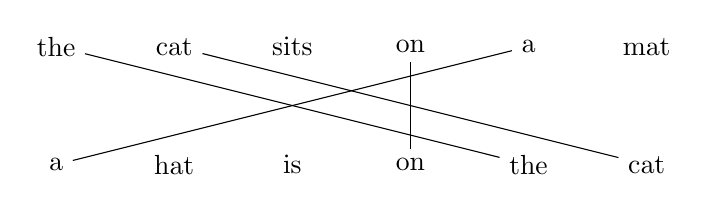
\begin{tikzpicture}[every node/.style={anchor=center}]
        % Sentence 1
        \node (w1) at (0,0) {the};
        \node (w2) at (1.5,0) {cat};
        \node (w3) at (3,0) {sits};
        \node (w4) at (4.5,0) {on};
        \node (w5) at (6,0) {a};
        \node (w6) at (7.5,0) {mat};

        % Sentence 2
        \node (v1) at (0,-1.5) {a};
        \node (v2) at (1.5,-1.5) {hat};
        \node (v3) at (3,-1.5) {is};
        \node (v4) at (4.5,-1.5) {on};
        \node (v5) at (6,-1.5) {the};
        \node (v6) at (7.5,-1.5) {cat};

        % Draw lines for exact matches
        \draw (w5) -- (v1); % "a"
        \draw (w4) -- (v4); % "on"
        \draw (w1) -- (v5); % "the"
        \draw (w2) -- (v6); % "cat"
    \end{tikzpicture}
    \caption[Exact matching module]{Exact matching module of \ac{meteor}. Intersections of matchings are called crossings.}
    \label{fig:meteor_crossings}
\end{figure}

Unigrams that have not yet been mapped are then eligible for alignment using the next module in order, such as Porter-stemmed matching or synonym matching, producing multiple sets of mappings between candidate and reference. 
From the resulting alignments, \ac{meteor} computes a weighted $\mathrm{F}$-score, as defined in \Cref{eq:meteor}. 
In this formulation, unigram precision $\operatorname{P}$ is the fraction of candidate unigrams that are mapped to reference unigrams relative to the total number of candidate unigrams. 
Conversely, unigram recall $\operatorname{R}$ is the fraction of candidate unigrams that are mapped to reference unigrams relative to the total number of reference unigrams~\citep{banerjee_METEOR_2005}.

\begin{equation}
    \operatorname{METEOR} = \operatorname{F_{mean}} = \frac{10  \operatorname{P}  \operatorname{R}}{\operatorname{R} + 9  \operatorname{P}}  (1 - \mathrm{Penalty})
\label{eq:meteor}
\end{equation}

The penalty function discourages fragmented alignments.
If bigram or longer matches are absent, the score is reduced by up to 50\%~\citep{banerjee_METEOR_2005}. 
Due to its sensitivity to lexical and semantic variation \ac{meteor} correlates more strongly with human judgments than \ac{bleu}, particularly at the sentence or segment level~\citep{zhou_paraphrase_2021,kurt_pehlivanoglu_comparative_2024}.


% \tikzstyle{startstop} = [rectangle, rounded corners, minimum width=3cm, minimum height=1cm,text centered, draw=black, fill=red!30]
% \tikzstyle{process} = [rectangle, minimum width=3cm, minimum height=1cm, text centered, draw=black, fill=blue!20]
% \tikzstyle{decision} = [diamond, minimum width=3cm, minimum height=1cm, text centered, draw=black, fill=green!30]
% \tikzstyle{arrow} = [thick,->,>=stealth]


% \begin{figure}[h!]
% \centering
% % \resizebox{\textwidth}{!}{%
% \begin{tikzpicture}[node distance=2.5cm, every node/.style={minimum width=3cm, minimum height=1cm, text centered, draw, fill=blue!20}]

% % Nodes in a circular layout
% \node (start) [rectangle, rounded corners, fill=red!30] at (90:4cm) {Candidate \& Reference Sentences};
% \node (matching) at (30:4cm) {Matching};
% \node (bestsubset) at (150:4cm) {Select Subset of Mappings};
% \node (fscore) at (180:4cm) {Compute F-Score};
% \node (end) [rectangle, rounded corners, fill=red!30] at (200:4cm) {$\operatorname{METEOR}$ Score};

% % Arrows
% \draw[->, thick] (start) -- (matching);
% \draw[<->, thick] (matching) -- (bestsubset);
% \draw[->, thick] (bestsubset) -- (fscore);
% \draw[->, thick] (fscore) -- (end);

% \end{tikzpicture}%
% % }
% \caption{Circular visualisation of $\operatorname{METEOR}$ score computation steps, from candidate and reference sentences to the final weighted F-score with penalty.}
% \label{fig:meteor_circular}
% \end{figure}


